\section{Single Parameter Families} 

\subsection{Exponential Family}

\subsection{Conjugate Priors}

\subsection{Computing Posteriors with Beta Prior and Binomial Likelihood}

  The motivation behind the Beta distribution is that it satisfies \textbf{conjugacy} with a binomial likelihood. That is, assume that we have some data $\mathbf{x}$ of $N$ observations containing $m$ successes and $N-m$ failures (note that this observation $\mathbf{x}$ was in a way "reduced" to the information of only the number of successes $m$). We assume that there is some true success rate $\theta$ (between $0$ and $1$, of course) coming from these samples, and our job is to try and guess the true rate to the best of our abilities.

  Before we even observe the data $\mathbf{x}$, our initial guess of $\theta$ might be modeled by the prior distribution $\theta \sim \text{Beta}(a, b)$. Furthermore, the likelihood is clearly a binomial (since it represents the probability of getting $m$ successes out of $N$ samples with fixed rate of success $\theta$), so $m\,|\,\theta \sim \text{Binomial}(N, \theta)$. With these conditions, we claim that the posterior is also a beta, since
  \begin{align*}
    p(\theta\,|\, m) & \propto p_\theta (\theta) \, p(m\,|\,\theta) \\
    & \propto \theta^{a - 1} (1 - \theta)^{b - 1} \cdot \theta^m (1 - \theta)^{N - m} \\
    & = \theta^{a + m - 1} (1 - \theta)^{b + N - m - 1}
  \end{align*}

\subsection{Bayesian Inference for Gaussian}

  The maximum likelihood framework gave point estimates for the parameters $\mu$ and $\Sigma$. Now we develop a Bayesian treatment by introducing prior distributions over these parameters. Given a set of $N$ $D$-dimensional observations $\mathbf{X} = \{x_1, \ldots, x_n\}$, the likelihood function is given by (the unnormalized function of $\mu$):
  \begin{equation}
    p(\mathbf{X}\,|\,\mu, \Sigma) = \prod_{n=1}^N p(x_n\,|\,\mu, \Sigma) = \frac{1}{(2\pi)^{D/2}} \frac{1}{|\Sigma|^{1/2}} \exp \sum_{n=1}^N \bigg(-\frac{1}{2} (x_n - \mu)^T \Sigma^{-1} (x_n - \mu)\bigg)
  \end{equation}

  The likelihood function takes the form of the exponential of a quadratic form in $\mu$. Thus, if we choose a prior $p(\mu)$ given by a Gaussian, it will be a conjugate distribution for this likelihood function. Taking our prior distribution to be
  \begin{equation}
    p(\mu, \Sigma) = \mathcal{N}(\mu, \Sigma\,|\,\mu_0, \Sigma_0)
  \end{equation}

  The similarity of the symbols $\mu, \Sigma$ with $\mu_0, \Sigma_0$ may be slightly confusing. We can think as such: $\mu, \Sigma$ are random variables that determine the parameters of some Gaussian distribution. But the values $\mu, \Sigma$ are uncertain, and their possible values with probabilities take the form of another distribution $\mathcal{N}(\mu_0, \Sigma_0)$. The posterior distribution is given by the familiar formula
  \begin{equation}
    p(\mu, \Sigma\,|\,\mathbf{X}) \propto p(\mathbf{X}\,|\,\mu, \Sigma) \; p(\mu, \Sigma)
  \end{equation}

  which is another Gaussian $p(\mu\,|\,\mathbf{X}) = \mathcal{N}(\mu, \Sigma\,|\, \mu_N, \Sigma_N)$. Let us place a few conditions for simplification. Since every Gaussian density can be represented as a product of independent univariate Gaussians, we can work with univariate Gaussians. Furthermore, let us assume that the true value of $\sigma$ is known, so all we have to do is find the posterior distribution of $\mu$ using the prior density $\mathcal{N}(\mu\,|\,\mu_0, \sigma_0^2)$. We have our prior and likelihood to be the following. Note that while the likelihood distribution is pretty much given, we have the flexibility to choose what our prior distribution is. We have only set the prior as a Gaussian simply because it is a conjugate form and therefore will greatly simplify calculations.

  \begin{align*}
    p(\mu) & = \mathcal{N}(\mu\,|\,\mu_0, \sigma_0^2) = \frac{1}{\sqrt{2 \pi \sigma^2}} \exp\bigg(-\frac{1}{2\sigma^2} (\mu - \mu_0)^2) \bigg) \\
    p(\mathbf{X}\,|\,\mu) & = \prod_{n=1}^N p(x_n\,|\,\mu) = \frac{1}{(2 \pi \sigma^2)^{N/2}} \exp\bigg(-\frac{1}{2 \sigma^2} \sum_{n=1}^N (x_n - \mu)^2 \bigg)
  \end{align*}

  which gives a posterior $p(\mu\,|\,\mathbf{X}) = \mathcal{N}(\mu \,|\, \mu_N, \sigma_N^2)$ where
  \begin{align*}
    \mu_N & = \frac{\sigma^2}{N \sigma_0^2 + \sigma^2} \mu_0 + \frac{N \sigma_0^2}{N \sigma_0^2 + \sigma^2} \mu_{ML} \\
    \frac{1}{\sigma_N^2} & = \frac{1}{\sigma_0^2} + \frac{N}{\sigma^2}
  \end{align*}

  and $\mu_{ML}$ is the maximum likelihood solution for $\mu$ given by the sample mean $\mu_{ML} = \frac{1}{N} \sum_{n=1}^N x_n$. These values make sense. We can see that the mean of the posterior distribution $\mu_N$ is a compromise between the prior mean $\mu_0$ and maximum likelihood solution $\mu_{ML}$. If the number of observed data points $N=0$, then it is simply the prior mean, but for $N \rightarrow \infty$, the posterior mean is given by the maximum likelihood solution since the data ``overpowers'' the prior mean assumption.

  Now, suppose that the mean of the Gaussian over the data is known and we wish to infer the variance. For convenience, let us work with the precision $\lambda = \frac{1}{\sigma^2}$ over the variance. The likelihood function for $\lambda$ is
  \begin{equation}
    p(\mathbf{X}\,|\,\lambda) = \prod_{n=1}^N \mathcal{N} (x_n\,|\, \mu, \lambda^{-1}) \propto \lambda^{N/2} \exp \bigg(-\frac{\lambda}{2} \sum_{n=1}^N (x_n - \mu)^2 \bigg)
  \end{equation}

  Note that since this is a function of $\lambda$, it behaves differently than the likelihood function of $\mu$, even though they are of the same form. Since the likelihood function is proportional to the product of a power of $\lambda$ and the exponential of a linear function of $\lambda$, we must find a prior distribution $p(\lambda)$ with precisely these proportional properties identical to that of the likelihood. Fortunately, the Gamma distribution satisfies them, defined by
  \begin{equation}
    p(\lambda\,|\,a_0, b_0) = \text{Gamma}(\lambda\,|\, a_0, b_0) = \frac{1}{\Gamma(a_0)} b_0^{a_0} \lambda^{a_0-1} \exp(-b_0 \lambda)
  \end{equation}

  Using Bayes rule and multiplying gives the posterior density
  \begin{equation}
    p(\lambda\,|\,\mathbf{X}) \propto \lambda^{a_0 - 1} \lambda^{N/2} \exp\bigg( -b_0 \lambda - \frac{\lambda}{2} \sum_{n=1}^N (x_n - \mu)^2 \bigg)
  \end{equation}

  which is indeed the density of a $\text{Gamma}(\lambda\,|\,a_N, b_N)$ distribution, where
  \begin{align*}
    a_N & = a_0 + \frac{N}{2} \\
    b_N & = b_0 + \frac{1}{2} \sum_{n=1}^N (x_n - \mu)^2 = b_0 + \frac{N}{2} \sigma_{ML}^2
  \end{align*}

  where $\sigma_{ML}^2$ is the maximum likelihood estimator of the variance. Now, suppose that both the mean and precision are unknown. To find a conjugate prior, we consider the dependence of the likelihood function on $\mu$ and $\lambda$.
  \begin{align*}
    p(\mathbf{X}\,|\,\mu, \lambda) & = \prod_{n=1}^N \bigg(\frac{\lambda}{2\pi}\bigg)^{1/2} \exp \bigg( -\frac{\lambda}{2} (x_n - \mu)^2 \bigg) \\
    & \propto \bigg(\lambda^{1/2} \exp \Big(-\frac{\lambda \mu^2}{2} \Big) \bigg)^N \, \exp \bigg( \lambda \mu \sum_{n=1}^N x_n - \frac{\lambda}{2} \sum_{n=1}^N x_n^2 \bigg)
  \end{align*}

  We now wish to identify a prior distribution $p(\mu, \lambda)$ that has the same functional dependence on $\mu$ and $\lambda$ as the likelihood function and that should therefore take the form
  \begin{align*}
    p(\mu, \lambda) & \propto \bigg( \lambda^{1/2} \exp \Big(-\frac{\lambda \mu^2}{2}\Big) \bigg)^\beta \exp\big( c \lambda \mu - d \lambda \big) \\
    & = \exp \bigg( -\frac{\beta \lambda}{2} \Big(\mu - \frac{c}{\beta} \Big)^2 \bigg) \, \lambda^{\beta/2} \exp \bigg(-\Big(d - \frac{c^2}{2\beta}\Big) \lambda \bigg)
  \end{align*}

  where $c, d, \beta$ are constants. Since we can always write $p(\mu, \lambda) = p(\mu\,|\,\lambda) p(\lambda)$, we can find $p(\mu\,|\,\lambda)$ and $p(\lambda)$ by inspection. We have just shown that $p(\mu \,|\, \lambda)$ is a Gaussian whose precision is a linear function of $\lambda$ and that $p(\lambda)$ is a gamma distribution, so the normalized prior takes the form
  \begin{equation}
    p(\mu, \lambda) = \mathcal{N}(\mu \,|\, \mu_0, (\beta\lambda)^{-1}) \; \text{Gamma}(\lambda\,|\,a, b)
  \end{equation}

  which is called the \textbf{Gaussian-Gamma distribution}. Note that this is not simply the product of an independent Gaussian prior over $\mu$ and a gamma prior over $\lambda$, because the precision of $\mu$ is a linear function of $\lambda$. The extension of this to multivariate random variables is straightforward.

\subsection{Inference over Periodic Distributions}

  Although Gaussian distributions are of great significance, there are situations in which they are inappropriate as density models for continuous variables (e.g. wind direction or quantities periodic over 24 hours). Such quantities are conveniently represented using an angular (polar) coordinate $0 \leq \theta < 2\pi$. Let us consider the problem of evaluating the mean of a set of observations $\mathbf{\theta} = \{\theta_1, \theta_2, \ldots, \theta_N\}$ of a periodic variable measured in radians. The simple average $(\theta_1 + \ldots + \theta_N)/N$ is strongly coordinate dependent. To find an invariant measure of the mean, we can see that the observations can be viewed as points on the unit circle and can therefore be described instead by two-dimensional unit vectors $x_1, \ldots, x_N$, where $x_n = (\cos{\theta_n}, \sin{\theta_n})$. We can average these vectors and compute its angle to find this average angle.

  \begin{equation}
    \overline{x} = \frac{1}{N} \sum_{n=1}^N x_n = \Big( \frac{1}{N} \sum_{n=1}^N \cos{\theta_n} , \frac{1}{N} \sum_{n=1}^N \sin{\theta_n} \Big) \implies \overline{\theta} = \tan^{-1} \bigg( \frac{\sum_{n=1}^N \sin{\theta_n}}{\sum_{n=1}^N \cos{\theta_n}} \bigg)
  \end{equation}

  In general, any distribution $p(\theta)$ that have period $2\pi$ must be defined such that it is nonnegative, integrate to $1$, and be periodic.
  \begin{align*} 
    p(\theta) & \geq 0 \\
    \int_0^{2\pi} p(\theta)\,d\theta  & = 1 \\
    p(\theta + 2\pi) & = p(\theta)
  \end{align*}

  We can obtain a Gaussian-like distribution that satisfies these three properties. Consider a 2-dimensional Gaussian over variables $x_1, x_2$ having mean $\mu = (\mu_1, \mu_2)$ and a covariance matrix $\Sigma = \sigma^2 I$. This gives us
  \begin{equation}
    p(x_1, x_2) = \frac{1}{2\pi \sigma^2} \exp \bigg( -\frac{(x_1 - \mu_1)^2 + (x_2 - \mu_2)^2}{2\sigma^2} \bigg)
  \end{equation}

  Now, suppose that we consider the value of this distribution along a circle of fixed radius. Then, this distribution will be periodic, although it will not be normalized. We can determine the form of this distribution by transforming from Cartesian coordinates to polar coordinates $(r, \theta)$ (so that $x_1 = r \cos{\theta}, x_2 = r \sin{\theta}$) and keeping $r$ constant.

  \begin{figure}[H]
    \centering
    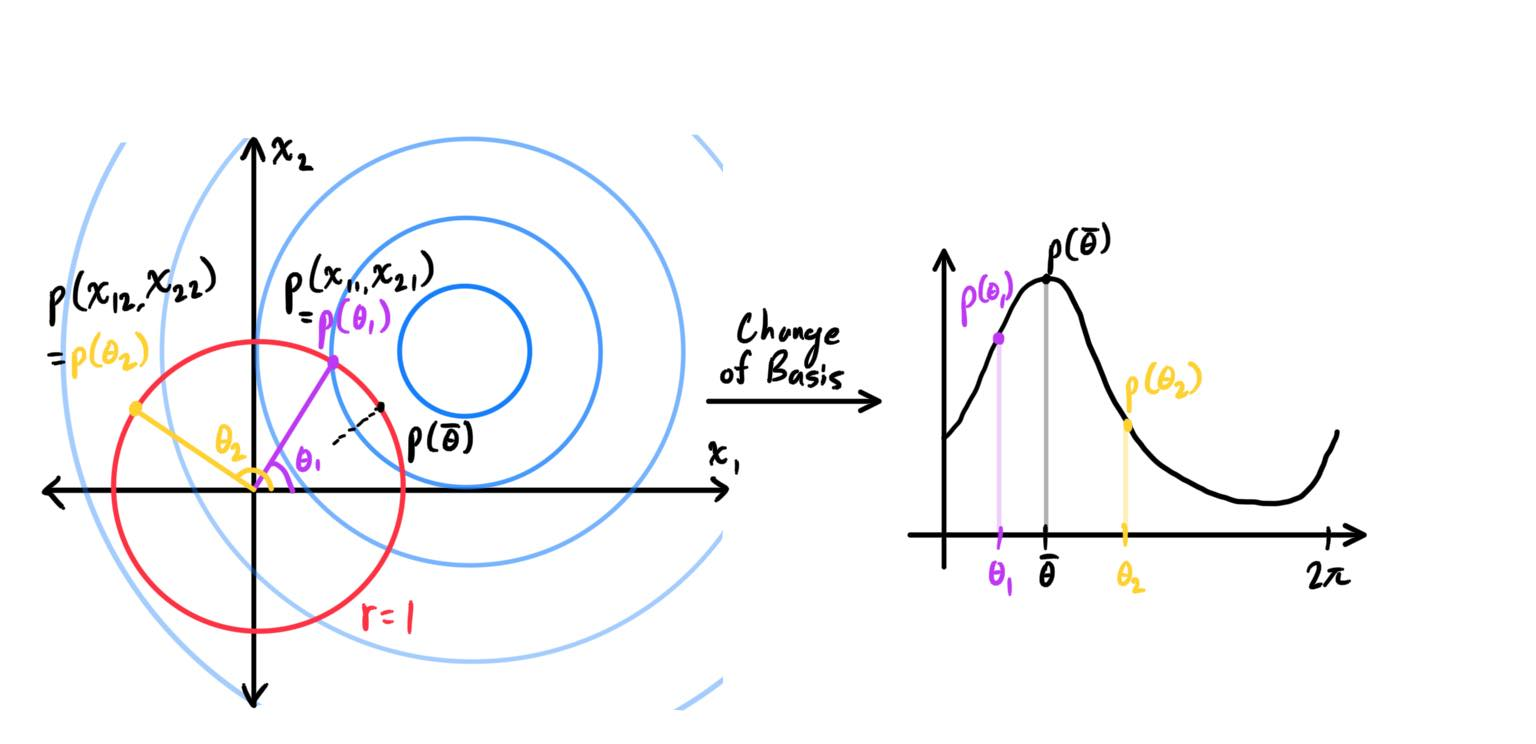
\includegraphics[width=0.7\textwidth]{img/circular_normal_change_of_basis.jpg}
    \caption{Circular normal change of basis}
  \end{figure}

  This transformation from $\mathbb{R}^2 \longrightarrow [0, 2\pi)$ defined
  \begin{equation}
    (x_1, x_2) \mapsto \tan^{-1} \frac{y}{x}
  \end{equation}
  simply takes the "circular" cross section of the Gaussian and maps those values.

  \begin{figure}[H]
    \centering
    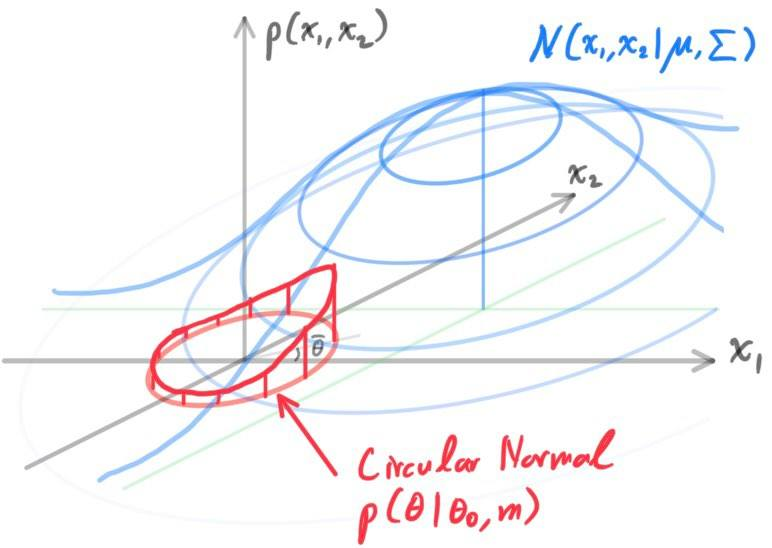
\includegraphics[width=0.5\textwidth]{img/Circular_Cross_Section.jpg}
    \caption{Circular cross section visualization}
  \end{figure}

  The value of $r$ is not important so we assume $r=1$. With some algebra and trig identities, we have the \textbf{circular normal}, or \textbf{von Mises distribution}, of form
  \begin{equation}
    p(\theta\,|\,\theta_0, m) = \frac{1}{2\pi I_0(m)} \exp \big( m \cos(\theta - \theta_0) \big)
  \end{equation}

  where the parameter $\theta_0$ corresponds to the mean of the distribution while $m$ is analogous to the precision for the Gaussian. The normalization coefficient $I_0(m)$ is the zeroth-order Bessel function of the first kind, defined by
  \begin{equation}
    I_0(m) = \frac{1}{2\pi} \int_0^{2\pi} \exp \big( m \cos{\theta}\big) \, d\theta
  \end{equation}

  For large $m$, the distribution becomes approximately Gaussian. Considering the maximum likelihood estimators for the parameters $\theta_0$ and $m$ for the circular normal, the log likelihood function is given by
  \begin{equation}
    \ln p(\mathbf{\theta}\,|\, \theta_0, m) = -N \ln(2\pi) - N \ln \big( I_0(m)\big) + m \sum_{n=1}^N \cos(\theta_n - \theta_0)
  \end{equation}

  The maximum estimator for the mean is
  \begin{equation}
    \theta_{0}^{ML} = \tan^{-1} \bigg( \frac{\sum_n \sin{\theta_n}}{\sum_n \cos{\theta_n}} \bigg)
  \end{equation}

  while that of $m$ can be evaluated numerically.

\subsection{Exponential Family of Distributions}

  The probability distributions so far are contained within the \textbf{exponential family} of distributions, which have important properties in common. The exponential family of distributions over $x \in \Omega \subset \mathbb{R}^D$, given parameters $\eta$, is defined to be the set of distributions of the form
  \begin{equation}
    p(x\,|\,\eta) = h(x) g(\eta) \exp\big(\eta^T u(x)\big)
  \end{equation}

  where $x$ may be a scalar or vector, discrete or continuous. Here, $\eta$ are called the \textbf{natural parameters} of the distribution, and $u(x)$ is some function of $x$. The function $g(\eta)$ can be interpreted as the normalizing coefficient and therefore satisfies
  \begin{equation}
    g(\eta) \int_{x \in \Omega} h(x) \exp\big(\eta^T u(x)\big) \, dx = 1
  \end{equation}

  with the integration replaced by a summation if $x$ is discrete.

  Now, consider a set of iid data denoted by $\mathbf{X} = \{x_1, \ldots, x_n\}$, for which the likelihood function is given by
  \begin{equation}
    p(X\,|\,\eta) = \bigg( \prod_{n=1}^N h(x_n) \bigg) g(\eta)^N\, \exp \bigg( \eta^T \sum_{n=1}^N u(x_n) \bigg)
  \end{equation}

  Setting the gradient of $\ln p(\mathbf{X}\,|\, \eta)$ with respect to $\eta$ to $0$, we can the following condition to be satisfied by the maximum likelihood estimator $\eta_{ML}$:
  \begin{equation}
    -\nabla \ln g(\eta_{ML}) = \frac{1}{N} \sum_{n=1}^N u(x_n)
  \end{equation}

  which can in principle be solved to obtain $\eta_{ML}$. The solution for the maximum likelihood estimator depends on the data only through $\sum_n u(x_n)$, which is therefore called the sufficient statistic of this distribution. Therefore, we do not need to store the entire data set itself but its sufficient statistic.

  In general, for a given probability distribution $p(\mathbf{X}\,|\, \eta)$, we can seek a prior that is conjugate to the likelihood function, so that the posterior distribution has the same functional form as the prior. Given that the likelihood function is in the exponential family, there exists a conjugate prior that can be written in the form
  \begin{equation}
    p(\eta) = p(\eta\,|\, \chi, \nu) = f(\chi, \nu) g(\eta)^\nu \exp \big( \nu \eta^T \chi \big)
  \end{equation}

  where $f(\chi, \nu)$ is a normalization coefficient, and $g(\eta)$ is the same function as the one appearing in the exponential family form of likelihood function. Indeed, multiplying this conjugate with the exponential family likelihood gives
  \begin{equation}
    p(\eta\,|\, \mathbf{X}, \chi, \nu) \propto g(\eta)^{\nu + N} \exp \Bigg( \eta^T \bigg( \sum_{n=1}^N u(x_n) + \nu \chi \bigg) \Bigg)
  \end{equation}


